\section{图的基本群}
\label{ch14-sec84}

现在我们来证明以下基本定理: 任何一个线性图的基本群都是自由群. 此后, 我们将简单地称线性图为\textbf{图}.

\begin{definition}[有向边、边道路]
\label{definition:ch14-oriented-edge}
图 $X$ 的一条\textbf{有向边}(oriented edge) $e$ 是 $X$ 的一条边和这条边的两个顶点的一个定向两者的总称, 顶点的定向中的第一个顶点叫做 $e$ 的\textbf{起始顶点}(initial vertex), 而第二个顶点叫做 $e$ 的\textbf{终结顶点}(final vertex). $X$ 中的\textbf{边道路}(edge path) 是 $X$ 中的有向边的一个序列 $e_{1}$, $\cdots$, $e_{n}$, 使得对于 $i=1$, $\cdots$, $n-1$, $e_{i}$ 的终结顶点等于 $e_{i+1}$ 的起始顶点. 这样一条边道路由序列 $x_{0}$, $\cdots$, $x_{n}$ 完全决定, 其中 $x_{0}$ 是 $e_{1}$ 的起始顶点, $x_{i}$ 是 $e_{i}$ 的终结顶点, $i=1$, $\cdots$, $n$. 它也被叫做从 $x_{0}$ 到 $x_{n}$ (from $x_{0}$ to $x_{n}$) 的边道路. 当 $x_{0}=x_{n}$ 时, 这条边道路叫做\textbf{闭的边道路}(closed edge path).

给定 $X$ 中的一条有向边 $e$, 令 $f_{e}$ 为从 $[0,\ 1]$ 到 $e$ 上的正线性映射, 这是从 $e$ 的起始顶点到 $e$ 的终结顶点的一条道路. 对应于从 $x_{0}$ 到 $x_{n}$ 的边道路 $e_{1}$, $\cdots$, $e_{n}$, 我们有一条通常意义下的从 $x_{0}$ 到 $x_{n}$ 的道路
\[
f=f_{1}*(f_{2}*(\cdots*f_{n})),
\]
其中 $f_{i}=f_{e_{i}}$. 这条道路是被边道路 $e_{1}$, $\cdots$, $e_{n}$ 唯一确定的, 我们称之为相应于边道路 $e_{1}$, $\cdots$, $e_{n}$ 的\textbf{道路}(path corresponding to the edge path). 如果边道路是闭的, 则相应的道路 $f$ 是一条回路.
\end{definition}

\begin{lemma}[图连通的边道路判别]
\label{lemma:ch14-connected-edge-path}
图 $X$ 是连通的当且仅当 $X$ 的每一对顶点能由 $X$ 中的一条边道路连接.
\end{lemma}

\begin{proof}
设 $X$ 是连通的. 如果 $X$ 中存在一条从 $x$ 到 $y$ 的边道路, 我们定义 $x\sim y$. $X$ 中的任何一条边的两个端点都是等价的. 记 $Y_{x}$ 为端点等价于 $x$ 的所有各边之并. 这时, $Y_{x}$ 是 $X$ 的一个子图, 从而在 $X$ 中是闭的. 各子图 $Y_{x}$ 将 $X$ 分割成无交的闭子空间. 由于 $X$ 是连通的, 这样的闭子空间应该只有一个.

反之, 设 $X$ 的每一对顶点能被某一条边道路连接. 这时每一对顶点也就能被通常意义下的道路连接. 因此 $X$ 的所有顶点属于 $X$ 的同一个分支. 由于每一条边都是连通的, 所以整条边也属于这个分支. 这证明 $X$ 是连通的.
\end{proof}

\begin{definition}[约化边道路与树]
\label{definition:ch14-reduced-tree}
设 $e_{1}$, $\cdots$, $e_{n}$ 是线性图 $X$ 中的一条边道路. 有时候会发生这样的情况: 对于某一个 $i$, $e_{i}$ 和 $e_{i+1}$ 是 $X$ 中边相同但定向相反的两条有向边. 如果不发生这种情况, 我们便称这条边道路为\textbf{约化边道路}(reduced edge path).

注意, 如果上面所说的情况确实发生了, 我们从这个有向边序列中删除 $e_{i}$ 和 $e_{i+1}$, 剩下来的还是一条边道路 (要先假定原来的序列中最少有三条边), 这个删除的过程叫做\textbf{约化边道路}. 因此我们可以说: 在任何连通图中, 每一对不同的顶点可以用一条约化边道路来连接. 参见\cref{ch14-fig-84-1}.

图 $X$ 的一个子图 $T$ 称为一棵\textbf{树}(tree), 如果 $T$ 是连通的并且没有闭的约化边道路.
\end{definition}

\par
\begin{figure}[htbp]
\centering
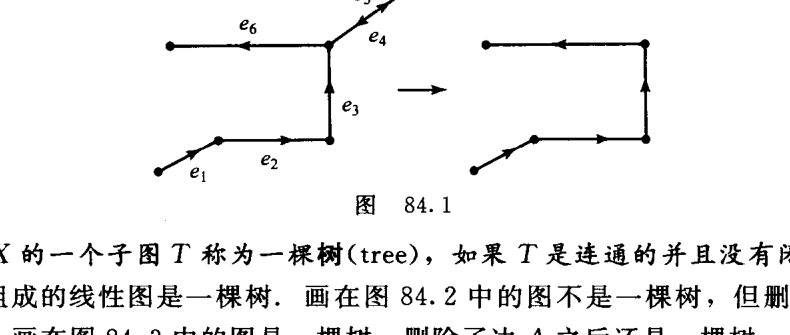
\includegraphics[width=0.7\textwidth]{image/fig-84-1.png}
\caption{边道路的约化.}
\label{ch14-fig-84-1}
\end{figure}

由一条边组成的线性图是一棵树. 画在\cref{ch14-fig-84-2} 中的图不是一棵树, 但删除了边 $e$ 之后便变成了一棵树. 画在\cref{ch14-fig-84-3} 中的图是一棵树, 删除了边 $A$ 之后还是一棵树.

\par
\begin{figure}[htbp]
\centering
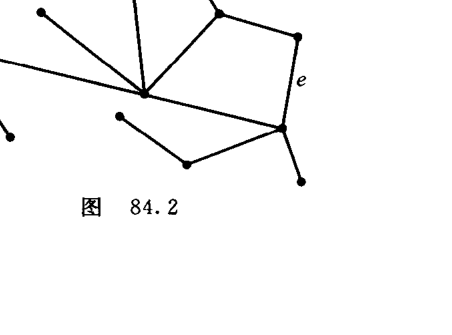
\includegraphics[width=0.45\textwidth]{image/fig-84-2.png}
\caption{非树 (删 $e$ 后为树).}
\label{ch14-fig-84-2}
\end{figure}

\par
\begin{figure}[htbp]
\centering
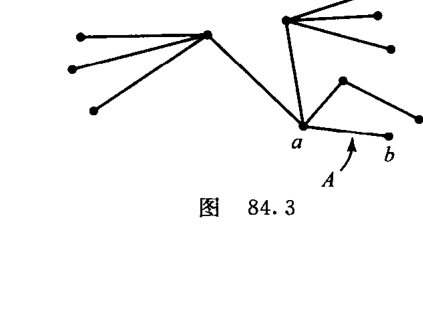
\includegraphics[width=0.45\textwidth]{image/fig-84-3.png}
\caption{树 (删 $A$ 后仍为树).}
\label{ch14-fig-84-3}
\end{figure}

\begin{lemma}[树的边扩张与分解]
\label{lemma:ch14-tree-extension}
如果 $T$ 是图 $X$ 中的一棵树, 并且 $A$ 是 $X$ 中的一条边, 它与 $T$ 恰相交于一个顶点, 则 $T\cup A$ 还是 $X$ 中的一棵树. 反之, 如果 $T$ 是 $X$ 中的一棵有限树, 由多于一条边构成, 则在 $X$ 中有一棵树 $T_{0}$ 和恰与 $T_{0}$ 相交于一个顶点的一条边 $A$, 使得 $T=T_{0}\cup A$.
\end{lemma}

\par
\begin{figure}[htbp]
\centering
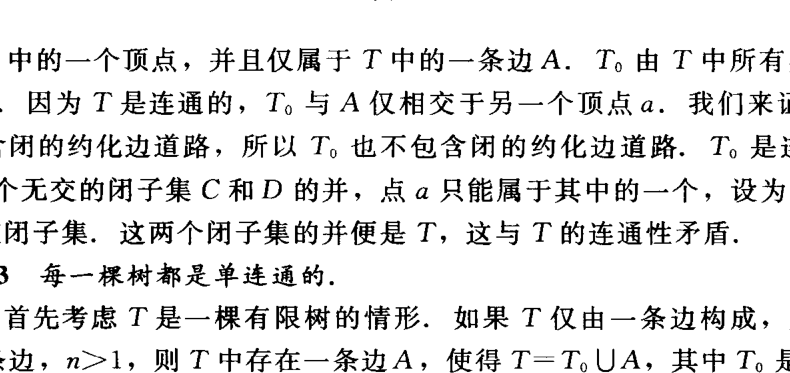
\includegraphics[width=0.7\textwidth]{image/fig-84-4.png}
\caption{有限树必具悬点.}
\label{ch14-fig-84-4}
\end{figure}

\begin{proof}
设 $T$ 是 $X$ 中的一棵树, $A$ 是与 $T$ 仅相交于一个顶点的一条边. 显然, $T\cup A$ 是连通的. 下面证明 $T\cup A$ 不包含闭的约化边道路. 设 $a$ 和 $b$ 是 $A$ 的两个端点, 并且 $\{a\}=T\cap A$. 参见\cref{ch14-fig-84-3}. 设 $x_{0}$, $\cdots$, $x_{n}=x_{0}$ 是 $T\cup A$ 中的一条闭的约化边道路的顶点序列. 如果没有一个顶点 $x_{i}$ 等于 $b$, 那么这条边道路便在 $T$ 中, 这与假设矛盾. 如果对于某一个 $i$, $0<i<n$, 使得 $x_{i}=b$, 则我们有 $x_{i-1}=a$ 和 $x_{i+1}=a$, 因此这条边道路不是约化的, 也与假设矛盾. 最后, 如果 $x_{0}=b=x_{n}$ 并且对于 $i=1$, $\cdots$, $n-1$, $x_{i}\neq b$, 则有 $x_{1}=a$ 和 $x_{n-1}=a$, 并且顶点序列 $x_{1}$, $\cdots$, $x_{n-1}$ 给出了 $T$ 中的一条闭的约化边道路, 还是与假设矛盾.

设 $T$ 是 $X$ 中多于一条边的一棵有限树. 首先我们证明 $T$ 中有某一个顶点 $b$ 只属于 $T$ 中的一条边. 如果不是这样, 我们在 $T$ 中构造一条边道路如下: 从 $T$ 的某一个顶点 $x_{0}$ 开始, 然后在 $T$ 中选取一条以 $x_{0}$ 为顶点的一条边 $e_{1}$. 给 $e_{1}$ 定向使得 $x_{0}$ 为起始顶点. 设 $x_{1}$ 为 $e_{1}$ 的另一个顶点, $e_{2}$ 是 $T$ 中以 $x_{1}$ 为顶点的不同于 $e_{1}$ 的一条边. 给 $e_{2}$ 定向使得 $x_{1}$ 为其起始顶点. 按照类似的方式继续下去. 在序列 $e_{1}$, $e_{2}$, $\cdots$ 中没有两个相邻的项是 $T$ 中的同一条边取不同定向. 由于 $T$ 是有限的, 应当有一个指标 $n$ 使得对于某一个 $i<n$ 有 $x_{n}=x_{i}$. 因此顶点序列 $x_{i}$, $x_{i+1}$, $\cdots$, $x_{n}$ 决定了 $T$ 中的一条闭的约化边道路, 这与假设矛盾. 参见\cref{ch14-fig-84-4}.


设 $b$ 是 $T$ 中的一个顶点, 并且仅属于 $T$ 中的一条边 $A$. $T_{0}$ 由 $T$ 中所有异于 $A$ 的边构成, 则 $T=T_{0}\cup A$. 因为 $T$ 是连通的, $T_{0}$ 与 $A$ 仅相交于另一个顶点 $a$. 我们来证明 $T_{0}$ 是一棵树. 由于 $T$ 不包含闭的约化边道路, 所以 $T_{0}$ 也不包含闭的约化边道路. $T_{0}$ 是连通的, 这是因为如果 $T_{0}$ 是两个无交的闭子集 $C$ 和 $D$ 的并, 点 $a$ 只能属于其中的一个, 设为 $C$, 于是 $C\cup A$ 和 $D$ 将会是无交闭子集. 这两个闭子集的并便是 $T$, 这与 $T$ 的连通性矛盾.
\end{proof}

\begin{theorem}[树是单连通的]
\label{theorem:ch14-tree-simply-connected}
每一棵树都是单连通的.
\end{theorem}

\begin{proof}
我们首先考虑 $T$ 是一棵有限树的情形. 如果 $T$ 仅由一条边构成, 则 $T$ 是单连通的. 如果 $T$ 有 $n$ 条边, $n>1$, 则 $T$ 中存在一条边 $A$, 使得 $T=T_{0}\cup A$, 其中 $T_{0}$ 是一棵有 $n-1$ 条边的树, 并且 $T_{0}\cap A$ 是一个顶点. 这时 $T_{0}$ 是 $T$ 的一个形变收缩核. 根据归纳假设 $T_{0}$ 是单连通的, 所以 $T$ 也是单连通的.

为了证明一般情形, 设 $f$ 是 $T$ 中的一条回路. $f$ 的像集是紧致的也是连通的, 所以它包含在 $T$ 的一个有限连通子图 $Y$ 中. 由于 $T$ 不包含闭的约化边道路, 所以 $Y$ 也不包含闭的约化边道路. 因此 $Y$ 是一棵树. 由于 $Y$ 是有限的, 所以它是单连通的. 因此 $f$ 在 $Y$ 中道路同伦于常值道路.
\end{proof}

\begin{theorem}[极大树的刻画]
\label{theorem:ch14-maximal-tree}
图 $X$ 中的一棵树 $T$ 是\textbf{极大的}(maximal), 如果 $X$ 中没有树以 $T$ 为真子集. 设 $X$ 是一个连通图. $X$ 中的一棵树 $T$ 是极大的当且仅当它包含 $X$ 的所有顶点.
\end{theorem}

\begin{proof}
设 $T$ 是 $X$ 中的一棵包含着 $X$ 的所有顶点的树. 如果 $Y$ 是 $X$ 的一个子图, 以 $T$ 为真子集, 我们来证明 $Y$ 包含着一条闭的约化边道路, 这样就证明了 $T$ 是极大的. 设 $A$ 是 $Y$ 的一条不在 $T$ 中的边, 根据假设, $A$ 的端点 $a$ 和 $b$ 都属于 $T$. 由于 $T$ 是连通的, 我们可以在 $T$ 中选取从 $a$ 到 $b$ 的一条约化边道路 $e_{1}$, $\cdots$, $e_{n}$. 如果在这个序列后面加上定向为从 $b$ 到 $a$ 的边 $A$, 便得到了 $Y$ 中的一条闭的约化边道路.

现在假设 $T$ 是 $X$ 中的一棵树, 它没有包含 $X$ 的所有顶点. 我们来证明 $T$ 不是极大的. 设 $x_{0}$ 是不在 $T$ 中的 $X$ 的一个顶点. 由于 $X$ 是连通的, 我们可以选取 $X$ 中从 $x_{0}$ 到 $T$ 中的某一个顶点的一条边道路, 把它写成顶点的序列 $x_{0}$, $\cdots$, $x_{n}$. 设 $i$ 是使得 $x_{i}\in T$ 的最小的指标. 令 $A$ 为 $X$ 中以 $x_{i-1}$ 和 $x_{i}$ 为顶点的边. 根据前一个引理, 这时 $T\cup A$ 是 $X$ 中的一棵树, 并且 $T\cup A$ 以 $T$ 为真子集.
\end{proof}

\begin{theorem}[极大树的存在性]
\label{theorem:ch14-maximal-tree-existence}
如果 $X$ 是一个线性图, 则 $X$ 中的每一棵树 $T_{0}$ 都包含在一棵极大的树中.
\end{theorem}

\begin{proof}
我们将 Zorn 引理应用于 $X$ 中所有包含 $T_{0}$ 的树构成的族 $\mathcal{T}$, 用严格的包含关系定义其中的偏序. 为了证明这个族有极大元, 只要证明以下论断:

如果 $\mathcal{T}'$ 是 $\mathcal{T}$ 中按严格包含关系而言的一个全序子族, 则 $\mathcal{T}'$ 中各成员之并 $Y$ 仍然是 $X$ 中的一棵树.

首先, 由于 $Y$ 是 $X$ 的某些子图的并, 它仍然是 $X$ 的一个子图. 其次, $Y$ 是包含着连通空间 $T_{0}$ 的一个族的并, 所以 $Y$ 是连通的.

最后, 我们假设 $e_{1}$, $\cdots$, $e_{n}$ 是 $Y$ 中的一条闭的约化边道路, 并且由此引出矛盾. 对于每一个 $i$, 选取 $\mathcal{T}'$ 中包含 $e_{i}$ 的一个成员 $T_{i}$. 由于 $\mathcal{T}'$ 按严格包含关系而言是全序, 所以树 $T_{1}$, $\cdots$, $T_{n}$ 中的某一个 (设为 $T_{j}$) 包含着其他的树. 于是 $e_{1}$, $\cdots$, $e_{n}$ 便是 $T_{j}$ 中的一条闭的约化边道路, 这与假设矛盾.
\end{proof}

现在我们来计算图的基本群. 需要以下结论.

\begin{lemma}[两点生成元]
\label{lemma:ch14-two-branch-generator}
设 $X=U\cup V$, 其中 $U$ 和 $V$ 都是 $X$ 中的开子集. 假设 $U\cap V$ 是道路连通的两个开子集 $A$ 和 $B$ 的无交并, $\alpha$ 是 $U$ 中从 $A$ 的点 $a$ 到 $B$ 的点 $b$ 的一条道路, 而 $\beta$ 是 $V$ 中从 $b$ 到 $a$ 的一条道路. 如果 $U$ 和 $V$ 都是单连通的, 则类 $[\alpha*\beta]$ 生成 $\pi_{1}(X,\ a)$.
\end{lemma}

\par
\begin{figure}[htbp]
\centering
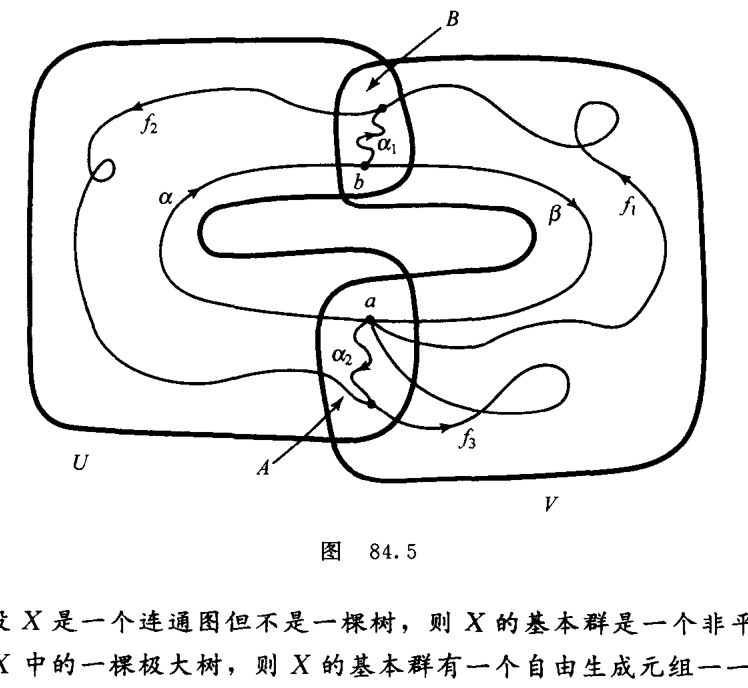
\includegraphics[width=0.7\textwidth]{image/fig-84-5.png}
\caption{$U\cap V$ 有两个道路分支的 van Kampen 情形.}
\label{ch14-fig-84-5}
\end{figure}

\begin{proof}
该情况类似于定理 59.1, 只是那里要求 $U\cap V$ 是道路连通的, 这里 $U\cap V$ 可以有两个道路连通分支. 证明也是类似的.

设 $f$ 是 $X$ 中以 $a$ 为基点的一条回路. 选取 $[0,\ 1]$ 的一个分拆 $0=a_{0}<a_{1}<\cdots<a_{n}=1$ 使得对于每一个 $i$, $f(a_{i})\in U\cap V$, 并且 $f$ 将 $[a_{i-1},\ a_{i}]$ 映射到 $U$ 或者 $V$ 中. 设 $f_{i}$ 是从 $[0,\ 1]$ 到 $[a_{i-1},\ a_{i}]$ 上的正线性映射与 $f$ 的复合. 于是 $[f]=[f_{1}]*\cdots*[f_{n}]$. 对于 $i=1$, $\cdots$, $n-1$, 在 $A$ 或者 $B$ 中选取一条从 $a$ 或 $b$ 到 $f(a_{i})$ 的道路 $\alpha_{i}$, 此外选取 $\alpha_{0}$ 和 $\alpha_{n}$ 为 $a$ 点处的常值道路. 设
\[
g_{i}=\alpha_{i-1}*(f_{i}*\alpha_{i}).
\]
经由直接计算可见, $[f]=[g_{1}]*\cdots*[g_{n}]$. 因为 $g_{i}$ 是 $U$ 或者 $V$ 中以集合 $\{a,\ b\}$ 中的点为端点的道路, 又因为 $U$ 和 $V$ 都是单连通的, 所以 $g_{i}$ 道路同伦于常值道路或者 $\alpha$, $\beta$, $\overline{\alpha}$, $\overline{\beta}$ 之一. 由此推出, $[f]$ 或者是平凡的, 或者等于 $[\alpha*\beta]$ 或者 $[\overline{\beta}*\overline{\alpha}]$ 的某正数次幂. 因此, $[\alpha*\beta]$ 生成群 $\pi_{1}(X,\ a)$. 参见\cref{ch14-fig-84-5}.

\end{proof}

\begin{theorem}[连通图的基本群是自由群]
\label{theorem:ch14-graph-fundamental-free}
设 $X$ 是一个连通图但不是一棵树, 则 $X$ 的基本群是一个非平凡的自由群. 事实上, 如果 $T$ 是 $X$ 中的一棵极大树, 则 $X$ 的基本群有一个自由生成元组一一对应于 $X$ 中那些不在 $T$ 中的边构成的族.
\end{theorem}

\par
\begin{figure}[htbp]
\centering
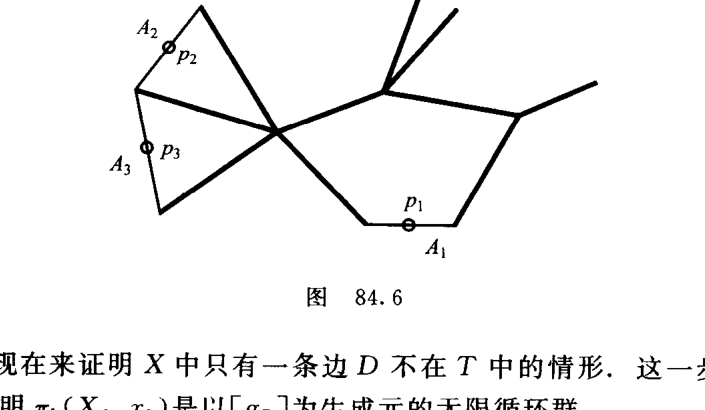
\includegraphics[width=0.7\textwidth]{image/fig-84-6.png}
\caption{有限归纳: 挖去内点作自由积.}
\label{ch14-fig-84-6}
\end{figure}

\par
\begin{figure}[htbp]
\centering
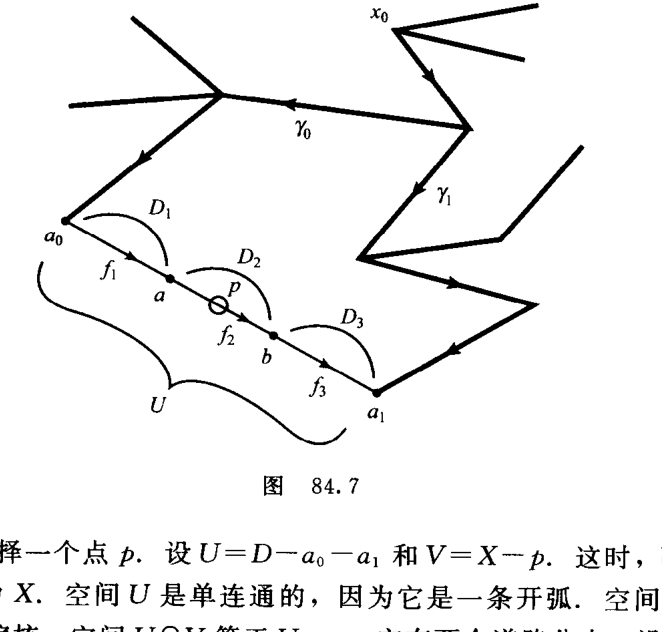
\includegraphics[width=0.65\textwidth]{image/fig-84-7}
\caption{单条非树边的情形.}
\label{ch14-fig-84-7}
\end{figure}

\begin{proof}
设 $T$ 是 $X$ 中的一棵极大树, 它包含着所有 $X$ 的顶点. 令 $x_{0}$ 为 $T$ 的一个固定的顶点. 对于 $X$ 的每一个顶点 $x$, 在 $T$ 中选取一条从 $x_{0}$ 到 $x$ 的道路 $\gamma_{x}$. 对于 $X$ 的每一条不在 $T$ 中的边 $A$, 在 $X$ 中定义一条回路 $g_{A}$ 如下: 首先, 给 $A$ 一个定向. 其次, 设 $f_{A}$ 为 $A$ 中从它的起始点 $x$ 到它的终结顶点 $y$ 的一条线性道路. 然后, 令
\[
g_{A}=\gamma_{x}*(f_{A}*\overline{\gamma}_{y}).
\]
我们来证明这些类 $[g_{A}]$ 形成 $\pi_{1}(X,\ x_{0})$ 的一个自由生成元组.

\textbf{第一步.} 我们先证明 $X$ 中的边只有有限条不在 $T$ 中的情形. 用归纳法. 归纳步骤是容易的, 所以把它放在前面.

设 $A_{1}$, $\cdots$, $A_{n}$ 为 $X$ 中不在 $T$ 中的那些边, 其中 $n>1$. 给这些边定向, 并且设 $g_{i}$ 表示回路 $g_{A_{i}}$. 对于每一个 $i$, 在 $A_{i}$ 的内部选取一个点 $p_{i}$. 设
\[
U=X-p_{2}-\cdots-p_{n}\qquad\text{和}\qquad V=X-p_{1}.
\]
这时, $U$ 和 $V$ 在 $X$ 中都是开的, 并且空间 $U\cap V=X-p_{1}-\cdots-p_{n}$ 是单连通的, 这是因为它以 $T$ 为形变收缩核. 因此, 根据推论 70.3, $\pi_{1}(X,\ x_{0})$ 是群 $\pi_{1}(U,\ x_{0})$ 和 $\pi_{1}(V,\ x_{0})$ 的自由积.

空间 $U$ 以 $T\cup A_{1}$ 为形变收缩核, 所以 $\pi_{1}(U,\ x_{0})$ 是以 $[g_{1}]$ 为生成元的自由群, 这一点我们将在第二步中证明. 根据归纳假设, 空间 $V$ 以 $T\cup A_{2}\cup\cdots\cup A_{n}$ 为形变收缩核, 所以 $\pi_{1}(V,\ x_{0})$ 是以 $[g_{2}]$, $\cdots$, $[g_{n}]$ 为生成元的自由群. 因此根据定理 69.2 可见, $\pi_{1}(X,\ x_{0})$ 是以 $[g_{1}]$, $\cdots$, $[g_{n}]$ 为生成元的自由群. 参见\cref{ch14-fig-84-6}.


\textbf{第二步.} 我们现在来证明 $X$ 中只有一条边 $D$ 不在 $T$ 中的情形. 这一步的证明要困难些. 给 $D$ 定向. 我们证明 $\pi_{1}(X,\ x_{0})$ 是以 $[g_{D}]$ 为生成元的无限循环群.

设 $a_{0}$ 和 $a_{1}$ 分别为 $D$ 的起始顶点和终结顶点. 将 $D$ 写成三条弧的并: $D_{1}$ 以 $a_{0}$ 和 $a$ 为端点, $D_{2}$ 以 $a$ 和 $b$ 为端点, $D_{3}$ 以 $b$ 和 $a_{1}$ 为端点. 参见\cref{ch14-fig-84-7}. 设 $f_{1}$, $f_{2}$ 和 $f_{3}$ 分别为 $D$ 中从 $a_{0}$ 到 $a$、从 $a$ 到 $b$ 和从 $b$ 到 $a_{1}$ 的线性道路. 以下应用前一个引理来计算 $\pi_{1}(X,\ a)$.


在弧 $D_{2}$ 的内部选择一个点 $p$. 设 $U=D-a_{0}-a_{1}$ 和 $V=X-p$. 这时, $U$ 和 $V$ 都是 $X$ 中的开集, 并且两者的并为 $X$. 空间 $U$ 是单连通的, 因为它是一条开弧. 空间 $V$ 是单连通的, 因为它以树 $T$ 为形变收缩核. 空间 $U\cap V$ 等于 $U-p$, 它有两个道路分支, 设 $A$ 为包含 $a$ 的那个分支, $B$ 为包含 $b$ 的那个分支. 这时前面引理中的假设条件得到满足. 道路 $\alpha=f_{2}$ 是 $U$ 中从 $a$ 到 $b$ 的一条道路. 如果我们记 $\gamma_{0}=\gamma_{a_{0}}$ 和 $\gamma_{1}=\gamma_{a_{1}}$, 则道路 $\beta=(f_{3}*(\overline{\gamma_{1}}*(\gamma_{0}*f_{1})))$ 是 $V$ 中从 $b$ 到 $a$ 的一条道路. 因此, $\pi_{1}(X,\ a)$ 由类
\[
[\alpha*\beta]=[f_{2}]*[f_{3}]*[\overline{\gamma_{1}}]*[\gamma_{0}]*[f_{1}]
\]
生成. 由此可见 $\pi_{1}(X,\ x_{0})$ 由类 $\widetilde{\delta}[\alpha*\beta]$ 生成, 其中 $\delta$ 是从 $a$ 到 $x_{0}$ 的道路 $\overline{f}_{1}*\overline{\gamma}_{0}$. 我们计算这个道路同伦类如下:
\[
\begin{aligned}
\widetilde{\delta}[\alpha*\beta]&=[\gamma_{0}*f_{1}]*[\alpha*\beta]*[\overline{f}_{1}*\overline{\gamma}_{0}]\\
&=[\gamma_{0}]*[f_{1}*(f_{2}*f_{3})]*[\overline{\gamma}_{1}]\\
&=[\gamma_{0}]*[f_{D}]*[\overline{\gamma}_{1}]\\
&=[g_{D}].
\end{aligned}
\]
因此, $[g_{D}]$ 生成 $\pi_{1}(X,\ x_{0})$.

接下来证明 $[g_{D}]$ 是无限阶的, 由此得到 $\pi_{1}(X,\ x_{0})$ 是一个无限循环群. 可以应用定理 63.1 (当时我们用它来证明 Jordan 曲线定理), 这个定理告诉我们 $[\alpha*\beta]$ 在 $\pi_{1}(X,\ a)$ 中是无限阶的. 也可以 (更简单些) 考虑映射 $\pi\colon X\to S^{1}$, 它将树 $T$ 映为一个点 $p$, 将开弧 Int $D$ 同胚地映到 $S^{1}-p$ 上. 这时, $\pi\circ\gamma_{0}$ 和 $\pi\circ\overline{\gamma}_{1}$ 都是常值道路, 所以
\[
\pi_{*}([g_{D}])=[\pi\circ f_{D}].
\]
这个类生成 $\pi_{1}(S^{1},\ p)$. 由此可见 $[g_{D}]$ 在 $\pi_{1}(X,\ x_{0})$ 中的阶是无限的.

\textbf{第三步.} 现在我们考虑 $X$ 有无限多条边不在 $T$ 中的情形. 这种情形下的证明十分类似于讨论无限圆周束时的证明, 所以我们略去细节. (参见定理 71.3.) 关键之处在于: 对于 $X$ 中任何一条以 $x_{0}$ 为基点的回路必有某一个有限指标 $\alpha_{i}$ 的集合, 使得这条回路在空间
\[
X(\alpha_{1},\cdots,\alpha_{n})=T\cup A_{\alpha_{1}}\cup\cdots\cup A_{\alpha_{n}}
\]
中, 并且任何这种回路之间的道路同伦也在这样的一个空间中. 根据这一点, 我们便能将一般情形化为有限情形.
\end{proof}

\begin{exercise}
\label{exercise:ch14-sec84-01}
举例说明引理 \cref{lemma:ch14-tree-extension} 的第二部分当 $T$ 无限时不必成立.
\end{exercise}

\begin{exercise}
\label{exercise:ch14-sec84-02}
计算 $n$ 个顶点的完全图和气水电图的基本群的自由生成元组的基数. (参见第 64 节.)
\end{exercise}

\begin{exercise}
\label{exercise:ch14-sec84-03}
设 $X$ 是两个圆周的束, $p\colon E\to X$ 是一个覆叠映射. $p_{*}$ 将 $E$ 的基本群同构地映到 $X$ 的基本群的子群 $H$ 上, 其中 $H$ 是两个生成元组 $\alpha$ 和 $\beta$ 生成的自由群.
\begin{enumerate}[(a)]
\item 对于第 81 节习题 2 中给出的四个覆叠空间 $E$, 确定 $E$ 的基本群的自由生成元组的基数.
\item 对于这些覆叠空间中的每一个, 通过 $\alpha$ 和 $\beta$ 表达出 $X$ 的基本群的子群 $H$ 的一个自由生成元组.
\end{enumerate}
\end{exercise}
